%\documentclass{report}
\documentclass{article}

\usepackage[left=5.5em, right=5.5em, top=8em]{geometry}
\usepackage{amsmath}
\usepackage{amssymb}
\usepackage{graphicx}
\usepackage{color}
\usepackage{listings}
\usepackage{hyperref}
\usepackage{fancyhdr}
\usepackage{tikz}
\usepackage{calc}
%\usepackage{svg}
\usepackage{graphicx,subcaption,lipsum}
\usepackage{nicefrac, xfrac}
\usepackage{enumitem}
\usepackage{listings}
\usepackage{xcolor}
\usepackage[parfill]{parskip}

\definecolor{backcolour}{rgb}{0.95,0.95,0.92}
\lstdefinestyle{mystyle}{backgroundcolor=\color{backcolour}}
\input{base/style.tex}
\date{}

\title{\vspace{10em}\textbf{Recherche de masque de transmission adapté à l'observation d'exoplanète à faible séparation} \\ \vspace{1.5em} \textsl{L'exemple de Proxima Centauri b} \vspace{5.5em} \\ \large{Stage encadré par Alexis Carlotti \& Lucie Leboulleux}}

% \makeatletter         
% \def\@maketitle{
% \raggedright
% 
\includegraphics[width = 30mm]{figures/logo_ipag.jpg}\\[2ex]
% \begin{center}
% {\huge  \@title }\\[4ex] 
% {\Large  \@author}\\[4ex] 
% \@date\\[8ex]
% \end{center}}
% \makeatother

\rhead{\large Rapport de stage — L2 Physique Recherche}
\lhead{\large IPAG - Laly Boyer - Mai/Juillet 2024}  


\setlength{\headheight}{14.0pt} % Increase headheight to 14.0pt
\lstset{style=mystyle}

\begin{document}
\maketitle
\vspace{5em}
\begin{center}
    \begin{minipage}{0.4\textwidth}
        \centering
        
\includegraphics[width = 25mm]{figures/logo_ipag.jpg}
    \end{minipage}
    \begin{minipage}{0.4\textwidth}
        \centering    
        
\includegraphics[width = 25mm]{figures/logo_uga.jpg}
    \end{minipage}
\end{center}
\thispagestyle{fancy}
\clearpage

\input{base/commandes.tex}
%
% Résumé de l'article
\begin{abstract}
Ceci est le résumé de mon article.
\end{abstract}

% Introduction
\section{Contexte}
Depuis la découverte de la première exoplanète en 1995, plus de 4000 exoplanètes ont été découvertes. Parmi elles, Proxima Centauri b, une exoplanète de type tellurique, est située dans la zone habitable de son étoile hôte, Proxima Centauri. Cette exoplanète est donc une cible privilégiée pour la recherche de signes de vie. Cependant, l'observation directe de cette exoplanète est rendue difficile par la faible séparation angulaire entre l'étoile et l'exoplanète. Il est donc nécessaire de développer des techniques d'observation adaptées pour pouvoir caractériser cette exoplanète. 

\section{Objectif}
Pour ceci, on se propose de rechercher un masque de transmission adapté à l'observation de Proxima Centauri b. L'objectif est de trouver un masque de transmission qui permet de réduire le flux de l'étoile tout en conservant le flux de l'exoplanète.

% % Contenu de l'article
% \section{Section 1}
% Contenu de la section 1.

% \section{Section 2}
% Contenu de la section 2.

% % Conclusion
% \section{Conclusion}
% Ceci est la conclusion de mon article.

\begin{abstract}
%L'enjeu
% La question de notre solitude dans l'univers s'est posé tout au long de l'existence de l'humanité, 
\item \paragraph{Introduction}
À la question \textsl{"Sommes-nous seuls dans l'univers ?"}, l'analyse et la caractérisation d'atmosphère d'exoplanètes pourrait bien y répondre. En effet, la recherche de vie ailleurs étant l'une des plus grandes questions astronomiques actuelles, ces domaines jouent un rôle crucial dans la compréhension de notre singularité dans l'univers. Proxima b, l'exoplanète la plus proche de notre système solaire, est une cible de choix pour ces études/recherches.

\vspace{-1.9em}
\item \paragraph{Objectif} 
Les exoplanètes potentiellement habitables sont généralement situé très proche de leurs étoiles (\textbf{Source ?}), autour de 1 unité astronomique (\textbf{Source ?}), et donc distinguer la lumière de ces planètes depuis la Terre demande de devoir déciphérer deux lumières à séparation angulaire très faible.

\vspace{-1.9em}
\item \paragraph{Méthodes}
La méthode que nous utiliserons ici pour surmonter ce problème est \textbf{l'apodisation}. On va venir modifier la lumière de l'étoile pour créer une zone de haut contraste, permettant de récupérer la lumière de la planète. Cela permettra d'analyser la lumière réfléchie de cette planète pour en déduire sa composition atmosphérique.

\vspace{-1.9em}
\item \paragraph{Résultats}
On a donc trouvé que l'apodiseur le plus optimal pour l'observation de Proxima b est un apodiseur de paramètres IWA = 2.6 OWA = 6.5 T = 0.70 sans bowtie. Cela permettra de gagner un certain temps de télescope, mais on est en définitive limité par un flou d'OA. Si on pouvait réduire ce flou jusqu'à $10^{??}$, alors on pourrait espérer augmenter le gain de SNR jusqu'à ???

\vspace{-1.9em}
\item \paragraph{Conclusion}
On sera toujours limité par le flou, faudrai améliorer le flou mais c'est chaud patate

% Je me repète complètement, c'est la même idée là mais j'aime bien les deux phrases quand meme :(

% En effet, ces planète étant généralement très proche de leurs étoiles (car leurs zone habitable sont de l’ordre de $$a=1\text{ UA}$$ comme la Terre en gros), et donc distinguer la lumière de la planète qui est 10^7 fois plus faible que celle de son étoile est un vrai challenge, au vu des distances angulaire à surmonter.

% %Ce qu'on sait déjà
% Une méthode pour surmonter ce problème est l’apodisation : on va venir créer une zone de haut contraste dans la lumière de l’étoile afin de permettre la récupération par l’instrument de la lumière de la planète, permettant de récupérer ces données et analyser la lumière réfléchis de cette planète pour analyser son atmosphere

% Les masques d’apodisations actuelles permettent d’observer jsuqu’a des 10-10 pour des planète assez éloigné et 10-5. Leurs paramètres sont (1.) IWA, (2.) OWA, (3.) T, et (4.) potentiel forme de la dark zone

% %Ce qu'on sait déjà - Limitation par le flou d'OA
% Nous verrons que bien que nous arrivons à atteindre de tes gros contraste, nous sommes limité par l’oa, qui vient créer un flou et limitant le contraste maximale atteignable par l’ELT-HARMONI, instrument sur lequel nous baserons nos recherche et simulation.

% %Méthodes
% À l’aide de simulation (1). réalisé dans l’approximation d’un flou d’optique adaptative uniforme dans notre champ de vue, et (2). d’une simulation plus réaliste avec de réels donnée de simulation d’OA, nous calculerons le gain en SNR des images de contrastes générés (PSF) pour une série d’apodiseur adéquat à l’observation de Proxima b.

% Pour ces deux situations, nous déterminerons le meilleur apodiseur

% Pour résumer, j’ai comparer des rapport de SNR d’apodiseur pour déterminer lequel était le meilleur pour l’observation de Proxima b

% - Il faut qu’il soit le plus grand possible (car $SNR^2$ = temps de téléscope en moins)

% - Il faut qu’il se trouve dans un certain intervalle de longueur d’onde

% - Il faut qu’on puisse récupérer toute l’information lumineuse de la planète pour toutes les longueurs d’onde d’observation

% %Résultats 
% Nous verrons qu’un masque optimal obtenu dans ce cadre de recherche correspond à un apodiseur de paramètres IWA = 2.6 OWA = 6.5 T = 0.70 sans bowtie 

% %Conclusion 
% On pourra donc gagner un certain temps de téléscope mais on est en définitive limité par un flou d’OA. Si on pouvait réduire le flou jusqu’à $10^(??)$, alors on pourrait espérer pouvoir augmenter le gain de SNR jusqu’à ???
\end{abstract}
%\section{Introduction}

\section{\centering Introduction - Proxima b et la recherche de vie ailleurs}
%Introduction ou contexte ? j'hésite
\setlength{\columnsep}{1.3em}%
\begin{wrapfigure}[15]{r}{0.45\textwidth}
    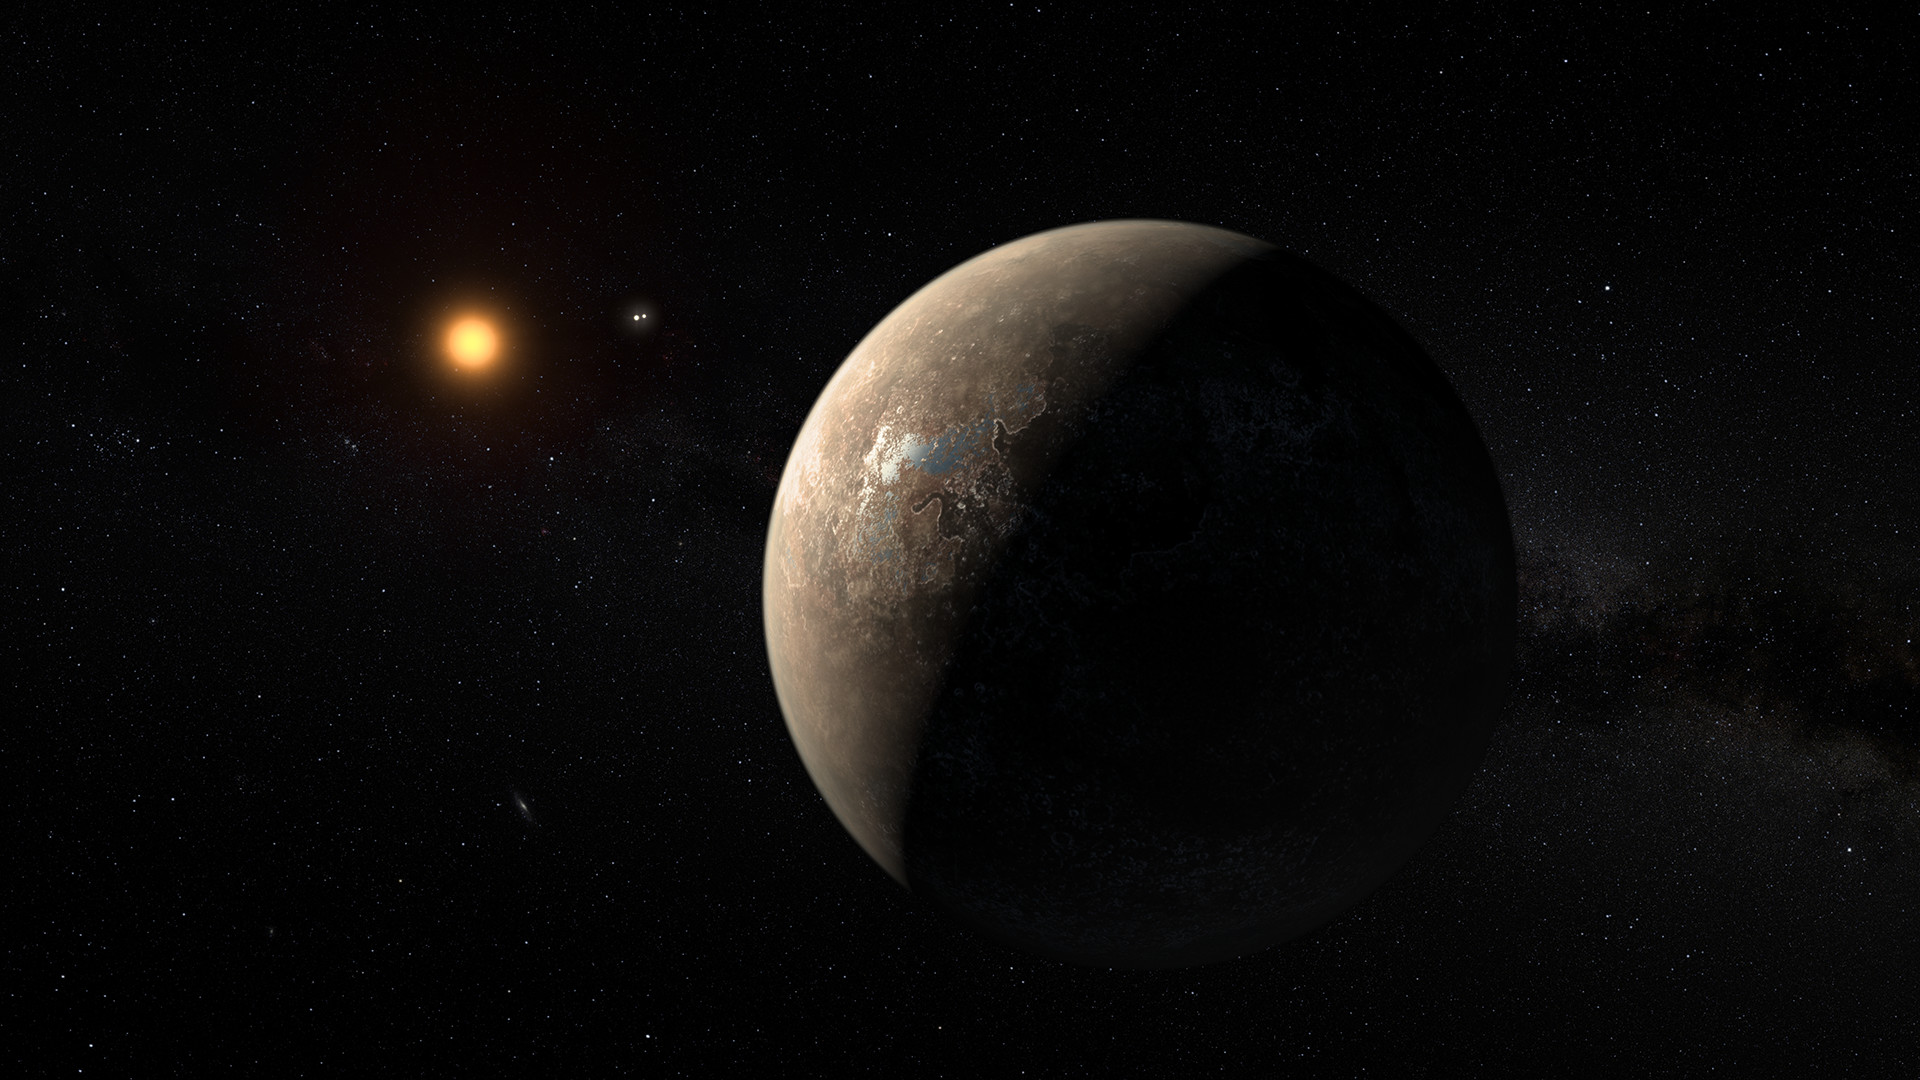
\includegraphics[width=0.45\textwidth]{figures/art_proxb.jpg}
    \caption{Vue d'artiste de Proxima Centauri b, l'exoplanète la plus proche de notre système solaire.}
\end{wrapfigure}

La recherche de planètes habitables a été identifié comme l'une des priorités majeures en astronomie selon le \textsl{Pathways to Discovery in Astronomy and Astrophyics for the 2020s} \cite{NAP26141}. En effet, la découverte de vie dans notre univers serait une avancée majeure pour l'humanité, et permettrait de répondre à des questions fondamentales sur notre place dans l'univers. 

Parmi les plus de 5000 exoplanètes découvertes à ce jour se trouve \textsl{Proxima b}, une exoplanète de type tellurique découverte en 2016, située dans la zone habitable de son étoile hôte Proxima Centauri. Étant donné sa proximité avec la Terre (à seulement 4.24 années-lumière), Proxima b est une cible de choix pour l'étude d'exoplanètes habitables. Non seulement son étude pourrait nous permettre de mieux comprendre les processus de formation et d'évolution des exoplanètes de type terrestres, mais la caractérisation de son atmosphère pourrait également nous permettre l'étude de potentielles biosignatures.

La possibilité de vie aussi proche de nous serait une découverte particulièrement marquante et symbolique pour l'humanité. \textsl{Proxima b} est donc une cible privilégiée pour la recherche de signes de vie. Cependant, son observation directe est rendue difficile par la faible séparation angulaire entre elle et son étoile. Située à une séparation angulaire de 37 mas, on pourrait comparer cela à la capacité de distinguer 2 objets à 6 mètres d'écart sur la Lune depuis la Terre. Il est donc nécessaire de développer des techniques d'observation adaptées pour pouvoir caractériser ce type d'exoplanètes proches de leurs étoile hôte.

Pour résoudre ce problème, l'ELT-HARMONI, un spectrographe de première lumière observant dans le visible et l'infrarouge (de 0.47 à 2.45 µm) prévu pour le télescope géant européen ELT, est équipé d'un Module Haut Contraste (HCM) développé à l'IPAG. Ce module permettra l'imagerie directe d'exoplanètes jusqu'à $10^{-6}$ fois plus faible que leur étoile hôte, et d'une séparation angulaire de 100 mas. Pour des raisons techniques (lesquels ?), l'observation est limité dans la bande H, soit entre 1.4 et 1.8 µm.

Bien qu'il existe des outils permettant d'observer des contrastes de l'ordre de $10^{-10}$ pour des planètes assez éloignées et $10^{-5}$ pour des planètes proches, ils sont limités par le flou d'\textsl{optique adaptative}. Ce flou, provoqué par le mouvement des miroirs venant corriger l'impact de l'atmosphère sur la lumière, limite le contraste maximal atteignable par l'ELT-HARMONI.

À l’aide de simulation réalisé dans l’approximation d’un flou d’optique adaptative uniforme dans notre champ de vue (1.), et d’une simulation plus réaliste avec de réels donnée de simulation d’OA (2.), nous calculerons le gain en SNR des images de contrastes générés (PSF) pour une série d’apodiseur adéquat à l’observation de Proxima b.

Pour ces deux situations, nous déterminerons le meilleur apodiseur, défini par le plus grand gain en SNR atteignable. En effet, plus grand est le gain en SNR, plus grand est le gain de temps de télescope, proportionnel au carré du gain en SNR.

%Conclusion 
% On pourra donc gagner un certain temps de téléscope mais on est en définitive limité par un flou d’OA. Si on pouvait réduire le flou jusqu’à $10^(??)$, alors on pourrait espérer pouvoir augmenter le gain de SNR jusqu’à ???


% En effet, ces planète étant généralement très proche de leurs étoiles (car leurs zone habitable sont de l’ordre de $$a=1\text{ UA}$$ comme la Terre en gros), et donc distinguer la lumière de la planète qui est 10^7 fois plus faible que celle de son étoile est un vrai challenge, au vu des distances angulaire à surmonter.

% %Ce qu'on sait déjà
% Une méthode pour surmonter ce problème est l’apodisation : on va venir créer une zone de haut contraste dans la lumière de l’étoile afin de permettre la récupération par l’instrument de la lumière de la planète, permettant de récupérer ces données et analyser la lumière réfléchis de cette planète pour analyser son atmosphere

% Les masques d’apodisations actuelles permettent d’observer jsuqu’a des 10-10 pour des planète assez éloigné et 10-5. Leurs paramètres sont (1.) IWA, (2.) OWA, (3.) T, et (4.) potentiel forme de la dark zone

% %Ce qu'on sait déjà - Limitation par le flou d'OA
% Nous verrons que bien que nous arrivons à atteindre de tes gros contraste, nous sommes limité par l’oa, qui vient créer un flou et limitant le contraste maximale atteignable par l’ELT-HARMONI, instrument sur lequel nous baserons nos recherche et simulation.

% %Méthodes
% À l’aide de simulation (1). réalisé dans l’approximation d’un flou d’optique adaptative uniforme dans notre champ de vue, et (2). d’une simulation plus réaliste avec de réels donnée de simulation d’OA, nous calculerons le gain en SNR des images de contrastes générés (PSF) pour une série d’apodiseur adéquat à l’observation de Proxima b.

% Pour ces deux situations, nous déterminerons le meilleur apodiseur

% Pour résumer, j’ai comparer des rapport de SNR d’apodiseur pour déterminer lequel était le meilleur pour l’observation de Proxima b

% - Il faut qu’il soit le plus grand possible (car $SNR^2$ = temps de téléscope en moins)

% - Il faut qu’il se trouve dans un certain intervalle de longueur d’onde

% - Il faut qu’on puisse récupérer toute l’information lumineuse de la planète pour toutes les longueurs d’onde d’observation

% %Résultats 
% Nous verrons qu’un masque optimal obtenu dans ce cadre de recherche correspond à un apodiseur de paramètres IWA = 2.6 OWA = 6.5 T = 0.70 sans bowtie 

% %Conclusion 
% On pourra donc gagner un certain temps de téléscope mais on est en définitive limité par un flou d’OA. Si on pouvait réduire le flou jusqu’à $10^(??)$, alors on pourrait espérer pouvoir augmenter le gain de SNR jusqu’à ???

% \subsection{Proxima et Proxima b, caractéristiques et intérêts d'observation}
% Résumé de l'article
% \begin{abstract}
% Ceci est le résumé de mon article.
% \end{abstract}

% Introduction
% \section*{Contexte}
% Depuis la découverte de la première exoplanète en 1995, plus de 5000 exoplanètes ont été découvertes. Parmi elles se trouve Proxima Centauri b, une exoplanète de type tellurique située dans la zone habitable de son étoile hôte, Proxima Centauri. Cette exoplanète est donc une cible privilégiée pour la recherche de signes de vie. Cependant, l'observation directe de cette exoplanète est rendue difficile par la faible séparation angulaire entre l'étoile et l'exoplanète. Il est donc nécessaire de développer des techniques d'observation adaptées pour pouvoir caractériser cette exoplanète.\\ 

% ELT-HARMONI est un spectrographe de première lumière observant dans le visible et l'infrarouge (de 0.47 à 2.45 µm) prévu pour le télescope géant européen ELT. Le Module Haut Contraste (HCM), développé à l'IPAG, permettra l'imagerie directe d'exoplanètes jusqu'à $10^{-6}$ fois plus faible que leur étoile hôte, et d'une séparation angulaire de 100 mas %\cite{SystemAnalysis} \cite{ZELDA}.

% \section*{Objectif}
% Pour ceci, on se propose de rechercher un masque de transmission adapté à l'observation de Proxima Centauri b. L'objectif est de trouver un masque de transmission qui permet de réduire le flux de l'étoile tout en conservant le flux de l'exoplanète.

% % Contenu de l'article
% \section{Section 1}
% Contenu de la section 1.

% %\Sfrac{1}{2}

% \section{Section 2}
% Contenu de la section 2.

% % Conclusion
% \section{Conclusion}
% Ceci est la conclusion de mon article.
\section{L'apodisation}

Le but de l'apodisation est de "lisser" un signal assez brut afin d'enlever ou adoucir les discontinuités sur ses bords. 
Cela va permetttre d'augmenter le contraste et de supprimer, du moins en partie, les anneaux de diffraction produits par un instrument d'optique, afin d'améliorer la définition des éléments à étudier.

\subsection{Bases sur la diffraction — Transformée de Fourier}

- La conversion pour comprendre comment on passe du plan pupille au plan focal
- graphe largeur commune et tout, avec condition que la planete soit visible a tout les longueur d’onde et que la largeur commune soit plus grand que le coeur de la PSF a la longueur d’onde max

Prenons l'exemple classique du signal d'une étoile, que l'on considèrera comme une source ponctuelle à l'infini, passant à travers l'ouverture circulaire d'un téléscope. 

On part d'une onde plane à l'infini qui passe à travers une ouverture circulaire. Lorsque l'onde atteint ce plan, elle devient alors une fonction circulaire $\text{circ}_r(\rho')$.
En passant par cette ouverture, la fonction circulaire devient par transformée de Fourier (c.f. \emph{Diffraction de Fraunhofer à l'infini}) la fonction de Bessel d'ordre 1 $J_1$ (Fig. 1.a), qu'on appelle aussi fonction "sombrero".

\begin{figure}[htbp]
    \centering
    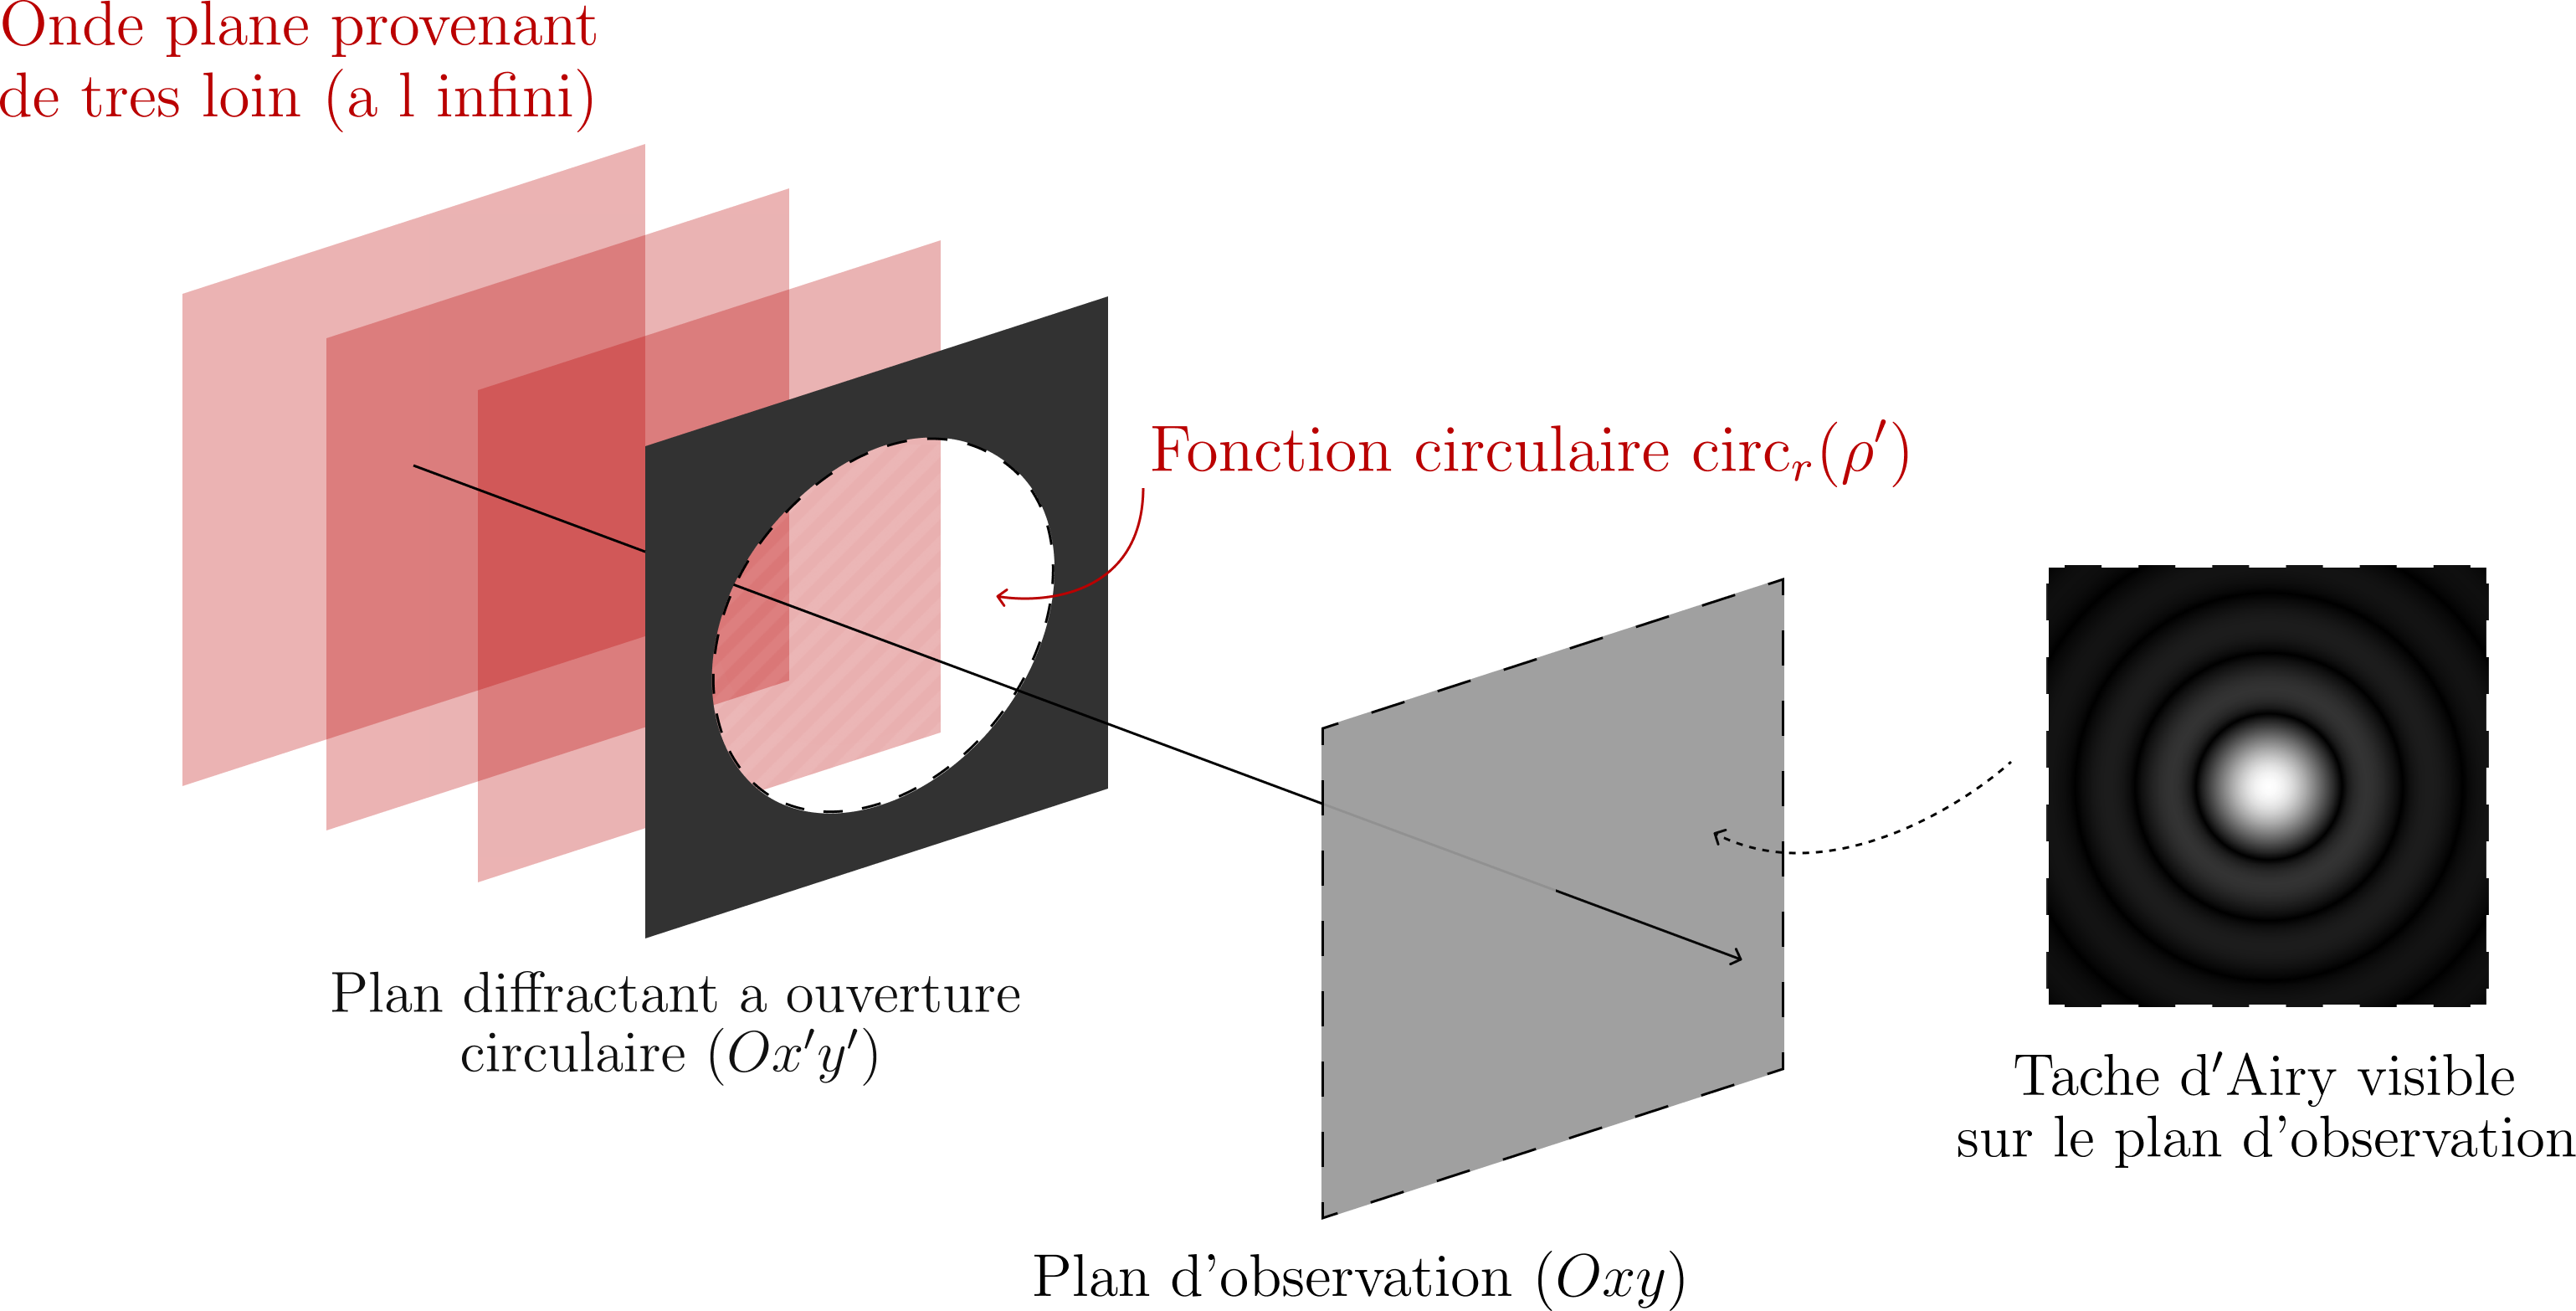
\includegraphics[width=0.75\textwidth]{figures/diff.png}
    \caption{Diffraction d'une onde plane par une ouverture circulaire.}
\end{figure}

Ce qu'on voit sur nos écrans lors des mesures est la \textbf{tâche d'Airy} (Fig 1.b), qui correspond à la fonction sombrero vue du dessus.

\begin{figure}[htbp]
    \centering
    \begin{subfigure}[b]{0.35\textwidth}
        \centering
        \includegraphics[width=\textwidth]{/Users/lalyboyer/Desktop/sombrr.png}
        \caption{Fonction de Bessel d'ordre 1 $J_1$, aussi appelé "fonction sombrero".}
    \end{subfigure}
    \hspace*{3cm}
    \begin{subfigure}[b]{0.35\textwidth}
        \centering
        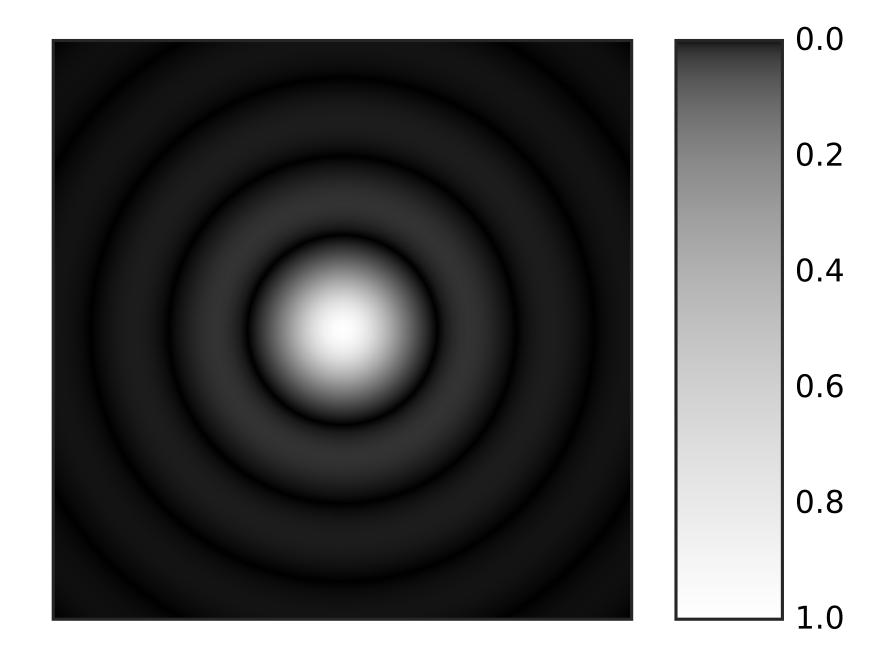
\includegraphics[width=\textwidth]{figures/airy_disk.png}
        \caption{Tâche d'Airy. L'intensité maximum de la tâche est atteinte en son centre, où est concentré la majorité de l'énergie.}
    \end{subfigure}
    \caption{Comparaison entre la fonction sombrero et la tâche d'Airy. On remarque que la tâche d'Airy correspond à la vue de dessus de la fonction $J_1$}
\end{figure}


Cette tâche d’Airy entraine toute une série d’implications pour l’imagerie, car une lentille n’est pas
infinie et limite la taille de l’onde. Cela entraine que l’image d’un point ne peut pas être un point mais
va être une tâche proportionnelle au rayon de la tâche d’Airy, ce rayon étant proportionnel à $\lambda$. %c’est ce qui explique que l’on peut mieux focaliser un laser bleu qu’un laser rouge
%et donc que le blue ray peut contenir plus d’information qu’un CD lu par un laser rouge.

Globallement, le centre de cette tâche (soit l'information compris dans le rayon $< 1.22\: \nicefrac{\lambda}{D}$) correspond à ce qu'on appelera le \textbf{coeur de la PSF} : l'essentiel de l'information qu'on peut récupérer à partir de la lumière de l'étoile se trouve dedans.



Ainsi, nous nous retrouvons à comprendre la nécessité de l'apodisation : la lumière diffracté de l'étoile va venir complétement recouvrir la lumière de l'exoplanète, rendant impossible l'analyse \iffalse ou genre récupérer l'information? \fi de la lumière de cette dernière. 

%Image montrant l'exemple

\begin{figure}[htbp]
    \centering
    \begin{subfigure}[b]{0.45\textwidth}
        \centering
        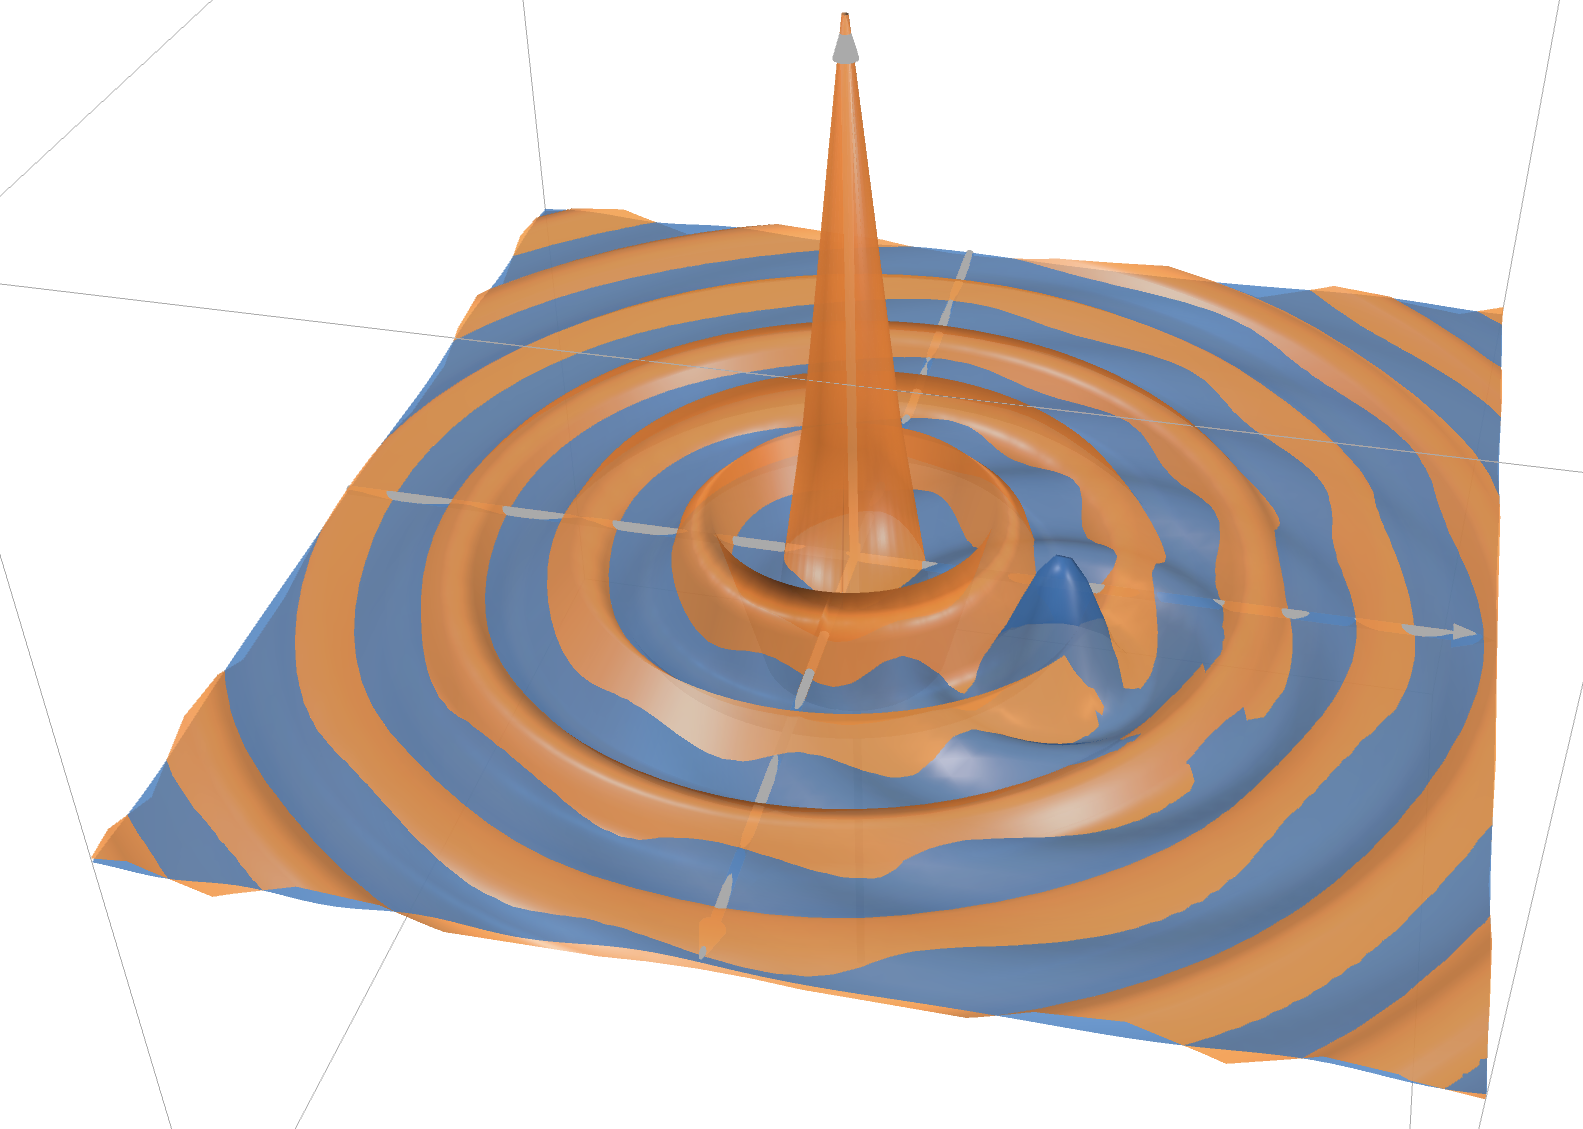
\includegraphics[width=\textwidth]{figures/st_pl_sgn.png}
        \caption{Zoomée sur la tâche d'Airy.}
    \end{subfigure}
    \hfill
    \begin{subfigure}[b]{0.45\textwidth}
        \centering
        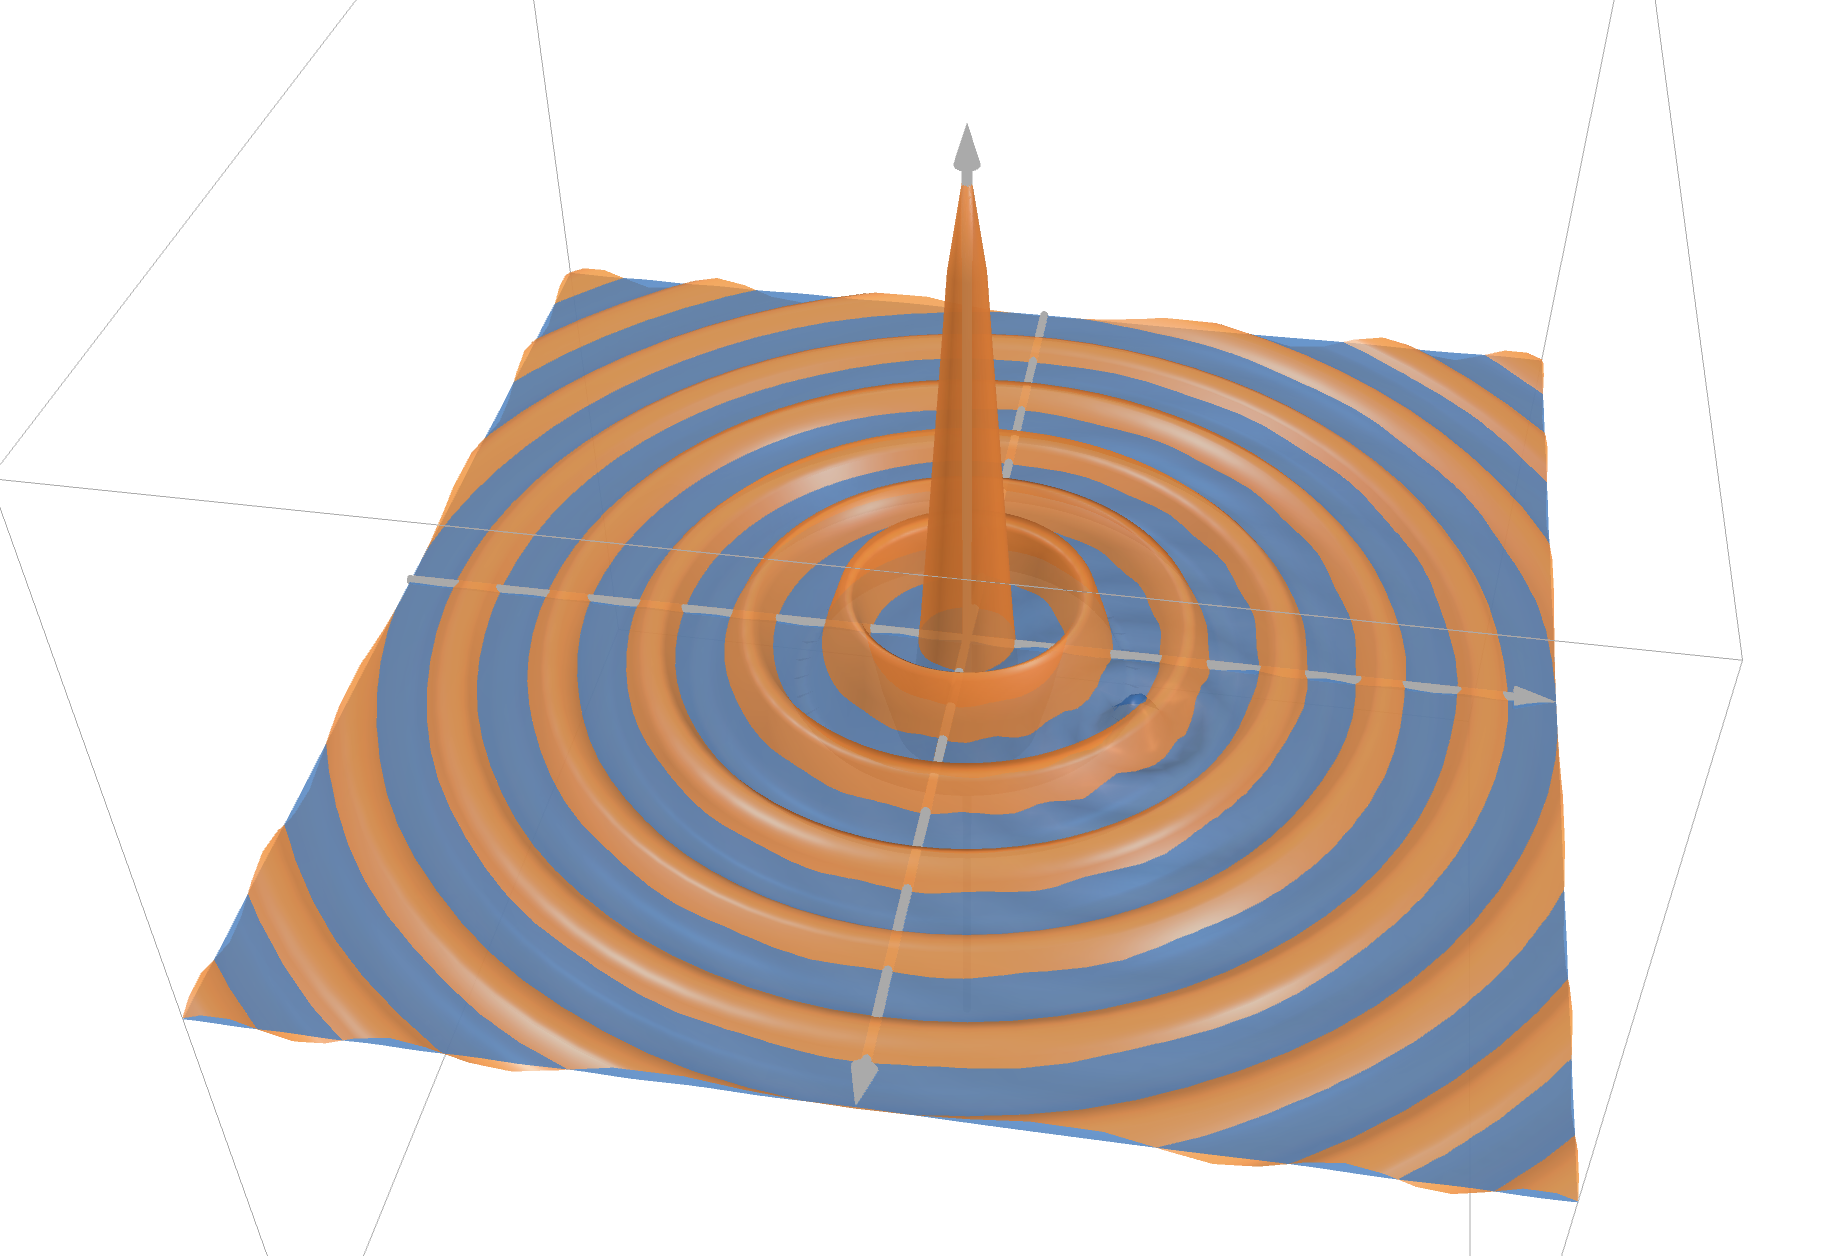
\includegraphics[width=\textwidth]{figures/larg_st_pl_sgn.png}
        \caption{Tâche d'Airy d'une exoplanète indistinguable de celle de l'étoile.}
    \end{subfigure}
    \caption{Exemple de la tâche d'Airy d'une étoile et de son exoplanète proche, avec (a) montrant un signal à peu près distinguable et en (b) le signal de l'exoplanète encore plus faible que l'exemple (a), rendant impossible la récupération de l'information de la planète.}
\end{figure}


Afin de pouvoir créer une zone de haut contraste permettant l'observation d'une exoplanète proche de son étoile, différentes méthodes sont possibles : nous choisirons ici l’apodisation à l’aide d’un \textbf{masque pupille}; nous allons commencer par définir ce dont il s'agit.

\subsection{Masque pupille — Apodiseur}

Un masque pupille (aussi appelé \emph{apodiseur}) est un carré en verre recouvert de chromium que l'on place dans le téléscope permettant de diffracter la lumière entrante dans le télescope de tel manière à pouvoir créer une zone où le contraste est suffisamment faible pour pouvoir observer des objets à luminosité très faibles autour d'objet très lumineux.

Ces masques permettent de diffracter la lumière autour de l’étoile afin de pouvoir créer une zone de haut contraste dans une zone souhaitée.

Illustration of the apodization technique in the focalplane. Top left: unapodized amplitude split into two shiftedamplitude (bottom left). The result of this coherent additionis the first-apodized amplitude (top center). This approachcan be iteratively reproduced: the split and shifted amplitudes(bottom center) and second-apodized amplitude (top right).

\begin{figure}[htbp]
    \centering
    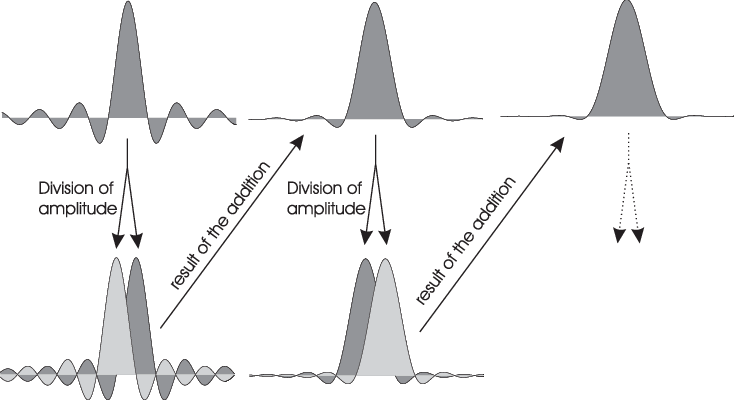
\includegraphics[width=0.7\textwidth]{figures/apod_explanation.png}
    \caption{Illustration de la technique d'apodisation dans le plan focal. En haut à gauche : amplitude non apodisée divisée en deux amplitudes décalées (en bas à gauche). Le résultat de cette addition cohérente est l'amplitude apodisée (en haut au centre). Cette approche peut être reproduite de manière itérative : les amplitudes divisées et décalées (en bas au centre) et l'amplitude apodisée (en haut à droite). }%\cite{apodExpl}}
\end{figure}

On peut ainsi remarquer qu'au fur et a mesure qu'on itère cette méthode, on crée une zone de haut contraste de plus en plus grande, permettant de récupérer de plus en plus d'information de l'exoplanète.

%Image montrant le principe physique de l'apodisation
Cependant, ce processus implique forcément une perte d'information, car la lumière de l'étoile est aussi diffractée. C'est pourquoi il est important de trouver un compromis entre la taille de la zone de haut contraste et la perte d'information.

En gros, on perd en résolution pour réduire la diffraction de l'étoile et augmenter le contraste de l'exoplanète.




% L’apodisation est une technique permettant de modifier la forme d’une fonction mathématique représentant un signal électrique, une transmission optique… de tel façon à enlever ou adoucir les discontinuités sur ces bords.
% Procédé destiné à augmenter le contraste et à supprimer, du moins en partie, les anneaux de diffraction produits par un instrument d'optique, afin d'améliorer la définition des éléments à étudier. [2.]

\begin{figure}[htbp]
    \centering
    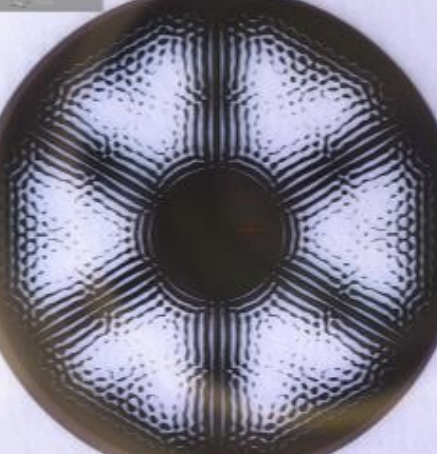
\includegraphics[width=0.3\textwidth]{figures/apod_harmoni.png}
    \caption{Apodiseur HC1 de l'instrument HARMONI.}%\cite{apod_harmoni}}
    %\label{fig:apod_harmoni}
\end{figure}
% L’apodisation est une technique permettant de modifier la forme d’une fonction mathématique représentant un signal électrique, une transmission optique… de tel façon à enlever ou adoucir les discontinuités sur ces bords.

% Procédé destiné à augmenter le contraste et à supprimer, du moins en partie, les anneaux de diffraction produits par un instrument d'optique, afin d'améliorer la définition des éléments à étudier. [2.]
\newpage
\section{\centering Point Spread Function}

\subsection{Définition}

La fonction d'étalement du point (= \textsl{Point Spread Function}), appelée \textbf{PSF}, est une fonction représentant la réponse d'un système optique à une source lumineuse ponctuelle. Dans notre cas, il s'agit de la réponse de l'optique de l'ELT à une étoile et son (ou ses) exoplanète(s).

Elle dépend de la longueur d'onde de la lumière observée, de la qualité de l'optique, de la turbulence atmosphérique, de la position de l'objet observé, etc... Pour la calculer, on calcule la transformée de Fourier en deux dimensions de la pupille de l'instrument. % * C'est pas la TF d'une source ponctuelle de 2D plutôt ? je comprends pas trop :/

\subsection{La PSF de la pupille de L’ELT}

Prenons l'exemple de la PSF d'une étoile à travers la pupille de l'ELT. En calculant la PSF d'une étoile à travers cette pupille, on obtient une forme particulière, qui dépend de la longueur d'onde observée.

\begin{figure}[htbp]
\centering
\begin{subfigure}[b]{0.40\textwidth}
\centering

\includegraphics[width=\textwidth]{figures/ELT_pupil.png}
\caption{Pupille de l'ELT. on peut voir les 6 araignées de l'ELT permettant de soutenir le miroir secondaire ainsi que le miroir secondaire y sont représenté. La partie blanche représentente les zones laissant passer la lumières.}
\label{fig:elt_pupil}
\end{subfigure}
\hfill
\begin{subfigure}[b]{0.46\textwidth}
\centering
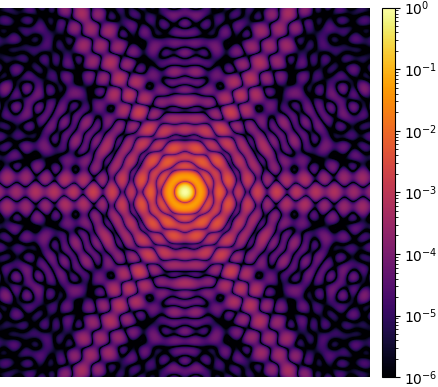
\includegraphics[width=\textwidth]{figures/PSF_ELT.png}
\caption{PSF normalisé de l'ELT représenté en échelle logarithme.}
\label{fig:pupil_diff}
\end{subfigure}
\caption{\textit{None}}
\end{figure}

On normalise la PSF pour que l'intensité lumineuse soit égale à 1 en son centre, et qu'on puisse voir l'image sous forme de contraste. Cela permet de mieux visualiser les zones où une exoplanète d'un certain contraste comparé à l'étoile serait potentiellement visible.

Dans la figure \ref{fig:pupil_diff}, on peut voir que l'on n'obtient pas exactement une fonction de Bessel d'ordre 1, mais une forme similaire avec un pic central et des anneaux de diffraction autour. Cette différence de forme est lié aux araignées de l'ELT et au miroir central qui viennent perturber la propagation de la lumière.

\begin{figure}[htbp]
\centering
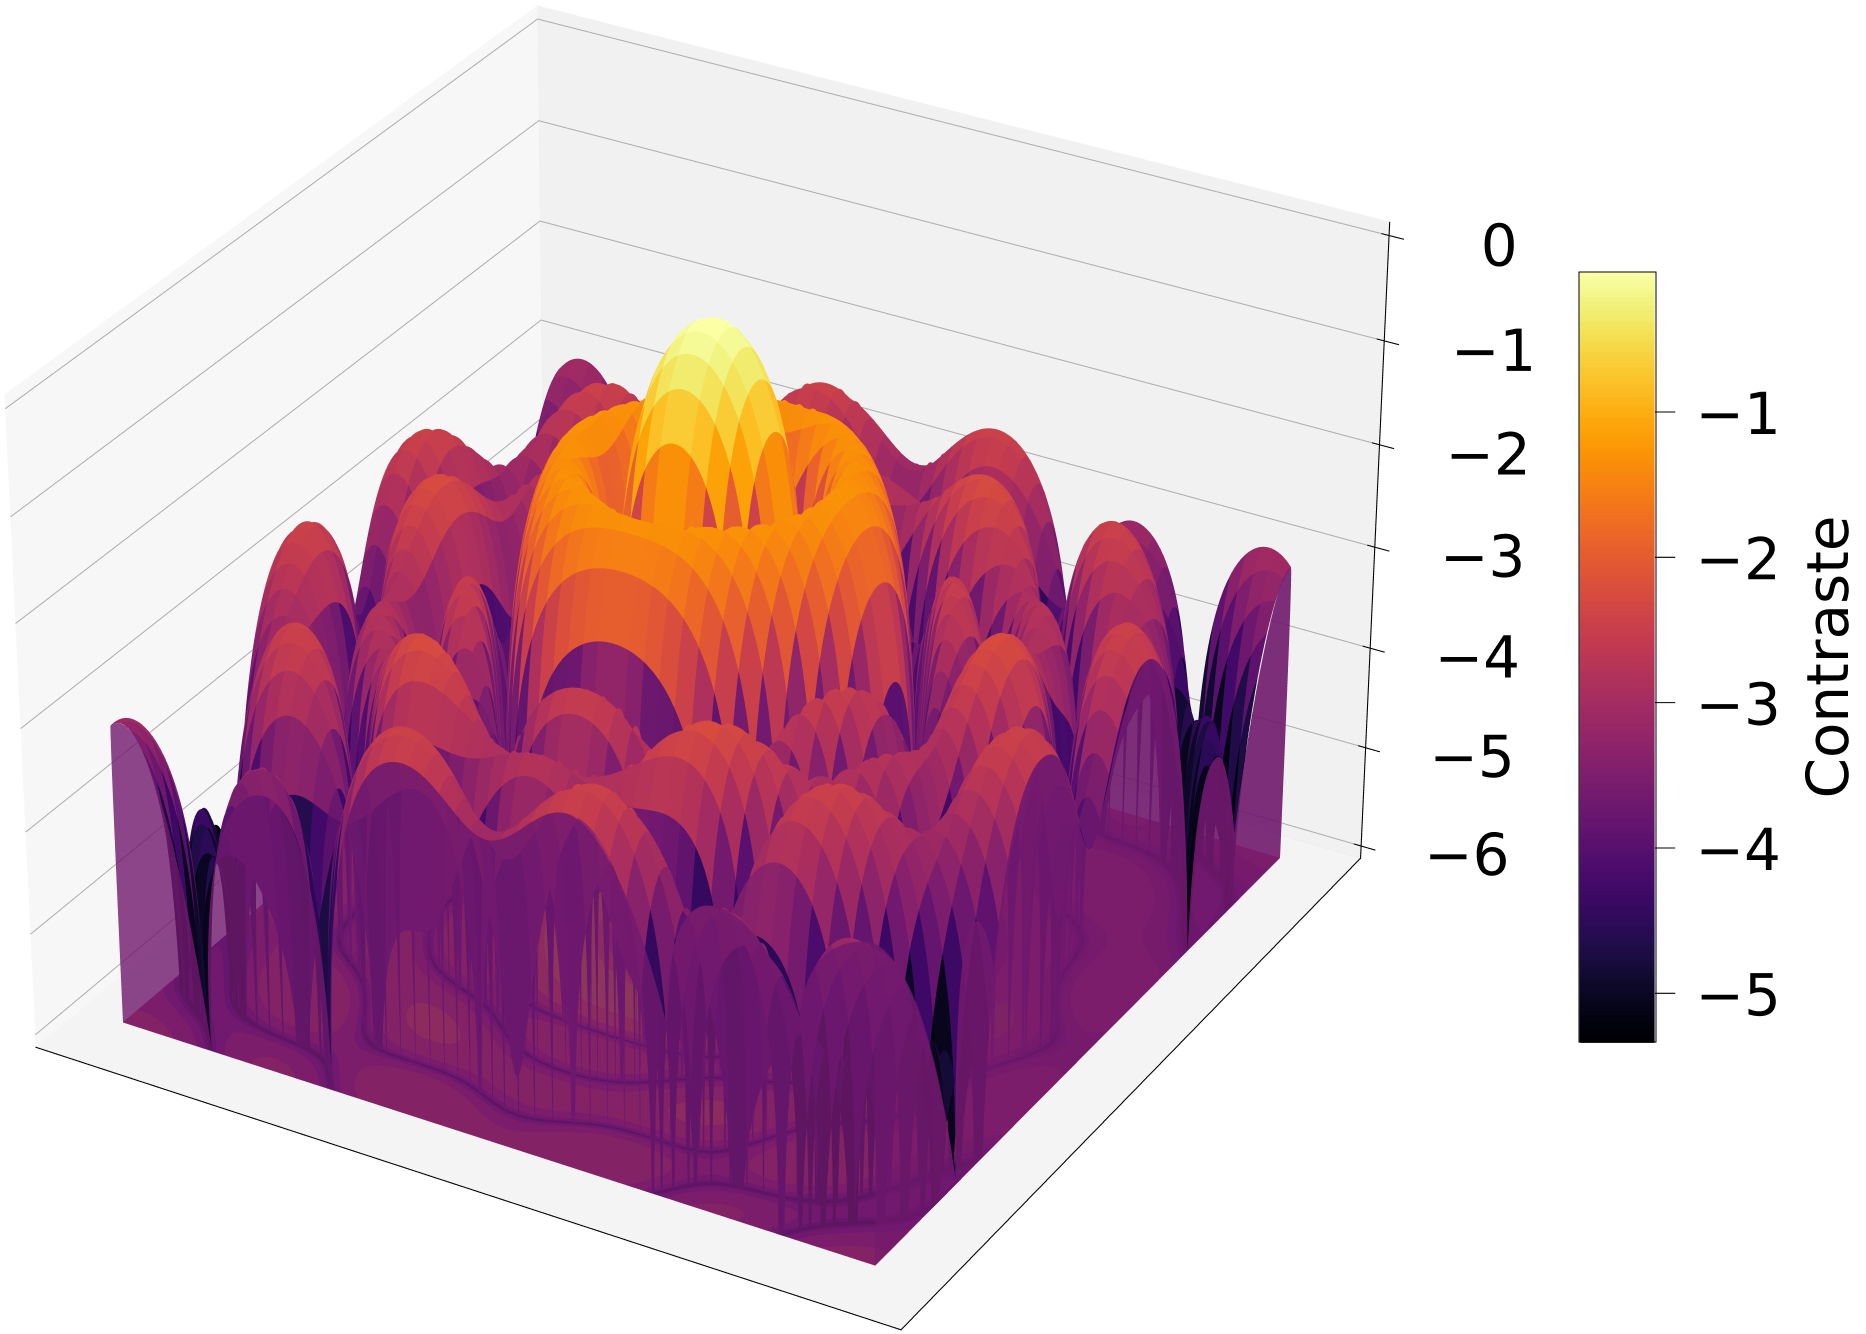
\includegraphics[width=0.7\textwidth]{figures/PSF_ELT_3D_bord.png}
\caption{Représentation 3D de la PSF normalisé de l'ELT représenté en échelle logarithme. On peut voir les anneaux de diffraction autour du pic central.}
\label{fig:3D_PSF}
\end{figure}


La représentation 3D de la PSF zoomée en échelle logarithme dans la figure \ref{fig:3D_PSF} permet de mieux se rendre compte des anneaux de diffraction, et des reliefs de contraste dans la PSF lié à la diffraction.

On se rend donc compte assez facilement de la difficulté de détecter la présence d'une exoplanète à faible séparation d'une étoile, car la PSF de l'étoile est bien trop intense comparé au contraste de l'exoplanète, qui sera trop faible en comparaison.


% comment on le calcule dans le code

\subsection{Exemple avec un apodiseur d'HARMONI}

Afin de visualiser les effets d'un apodiseur, nous pouvons nous reférer 
aux deux apodiseurs prévues pour le HCM : l'apodiseur SP1 \ref{fig:SP1}, dont l'objectif et de créer une zone de haut contraste proche de l'étoile, et l'apodiseur SP2 \ref{fig:SP2}, qui a pour but d'observer une zone beaucoup plus large mais moins proche de l'étoile. L'avantage de ces deux apodiseurs est qu'ils permettent à eux seuls l'observation d'un vaste champ de vue, permettant d'observer différents objets potentiellement présents autour d'étoiles. À 1.45 µm, SP1 permet d'observer de 42 mas à 89 mas, et SP2 de 57 mas à 295 mas, et pourront atteindre un contraste de $10^{-6}$.

On peut voir que les zones de hauts contrastes sont net et défini par 2 rayons limites : l'Inner Working Angle (IWA) et l'Outer Working Angle (OWA). Ces deux angles correspondent à la séparation angulaire minimum et maximum imposé dans lequel on souhaite créer la zone de haut contraste.
% In the latter case, the result is that planets with a flux ratio of 10−6 may be detected as close as 50mas from the star, and with a flux ratio of a few 10−7 at 100mas.
%A constraint was in fact set on the relative intensity of that light in a region than encompasses the whole FoV, so that this its mean value would not be higher than the maximum intensity of the AO halo in the high-contrast region, which may be as low as 10−4 in good seeing conditions (first quartile, 0.43”).
% * Les contrastes atteints par chacun ?

% ! An exploration of the parameter space (minimum and maximum separations, contrast, and throughput) concluded that a 35% throughput could be achieved while satisfying the robustness, contrast, and maximum separation requirements if the minimum separation was set to 7.3λ/D. By comparison, satisfying them for a 6λ/D minimum separation would result in a twice as low throughput. A 7.3λ/D minimum separation corresponds to a 96mas angular distance on sky, which satisfies the top-level requirement of HARMONI.

%The HCM is designed to observe in the H and K bands. Since the PSF scales with the wavelength, it is necessary to use two FPM for each apodizer, unless the minimum separation of one in the H band corresponds to the minimum separation of the other in the K band, in which case only three FPM are required in total, and this solution was chosen given the limited number of available FPM.

On remarque que l'apodiseur SP2 à l'air plus fragmenté comparé au SP1; cela est du à la différence de fréquence spatiale apodisé : plus on cherche à créer une zone de haut contraste éloigné du centre, plus les fréquence spatiale à diffracté seront ??? et plus l'apodiseur sera 'fragmenté'. % * je sais plus exactement comment ça marche :p

\begin{figure}[htbp]
\centering
% Première ligne avec SP1
\begin{subfigure}[b]{0.40\textwidth}
\centering

\includegraphics[width=\textwidth]{figures/SP1_HARMONI.png}
\caption{Apodiseur SP1 de HARMONI-ELT.}
\label{fig:SP1}
\end{subfigure}
\hfill % Espace entre les images
\begin{subfigure}[b]{0.45\textwidth}
\centering
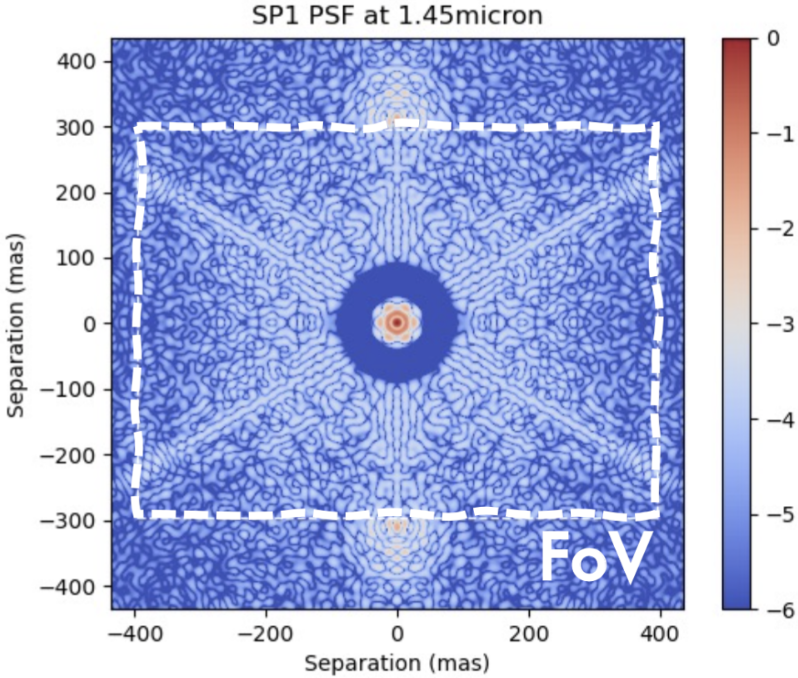
\includegraphics[width=\textwidth]{figures/PSF_SP1_HARMONI.png}
\caption{PSF SP1 de HARMONI-ELT.}
\label{fig:PSF_SP1}
\end{subfigure}
% Deuxième ligne avec SP2
\begin{subfigure}[b]{0.40\textwidth}
    \centering
    
\includegraphics[width=\textwidth]{figures/SP2_HARMONI.png}
    \caption{Apodiseur SP2 de HARMONI-ELT.}
    \label{fig:SP2}
\end{subfigure}
\hfill % Espace entre les images
\begin{subfigure}[b]{0.45\textwidth}
    \centering
    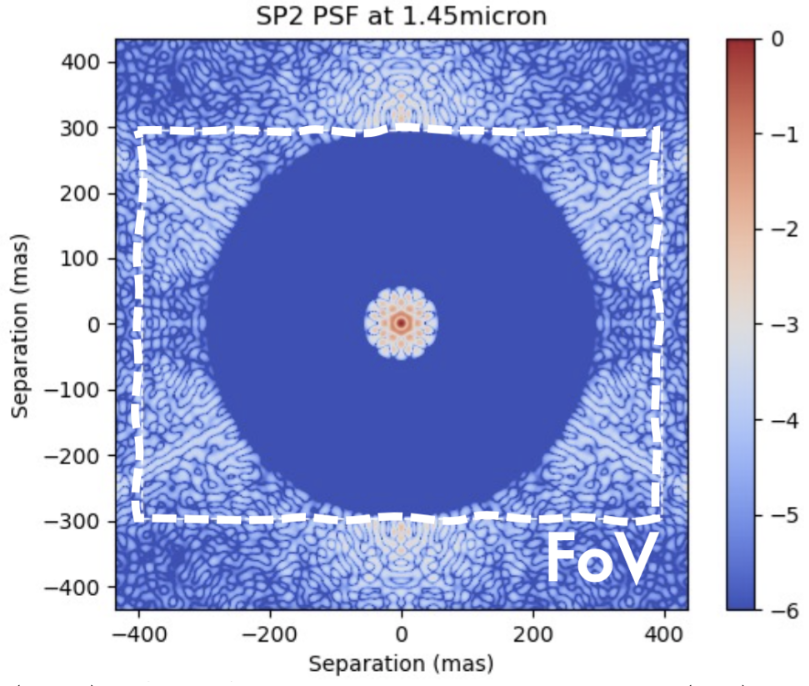
\includegraphics[width=\textwidth]{figures/PSF_SP2_HARMONI.png}
    \caption{PSF SP2 de HARMONI-ELT.}
    \label{fig:PSF_SP2}
\end{subfigure}

\caption{\textit{Comparaison des apodiseurs et des PSF pour SP1 et SP2 de HARMONI-ELT.}}
\end{figure}

\subsection{Nyquist}

On rappelle la définition de la fréquence de Nyquist : c'est la fréquence maximale que l'on peut observer dans un signal échantillonné. Elle est égale à la moitié de la fréquence d'échantillonnage.

Dans notre cas, cela signifie que pour observer correctement une planète, il faut que la planète soit échantillonnée par au moins 2 pixels par $\lambda/D$.

On présente 3 cas :

- On se trouve en dessous de Nyquist

Pas assez de données, on peut pas correctement analyser les données et affirmer ce qu'on voit (planète ou pas)

- On se trouve au dessus de Nyquist, on peut voir la planète
au moins 2 pixels par lambda/D
- On se trouve au dessus de Nyquist
temps de calcul trop long
- On se trouve à Nyquist

on peut voir la planète et analyser les données sans que ça prenne trop de temps de calcul

\section{\centering Optique Adaptative}

- prise en compte d’un “flou” qu’on peut considérer constant car on est tres proche sur un intervalle très court
- prise en compte de l’optique adaptative

\subsection{Intégration de l’OA dans nos PSF}

- TF et l’exponentiel qui dépend de la longueur d’onde :P
\section{SNR}
\subsection{Définition du SNR}

- pas oublier l’erreur que j’ai fait un moment de pas considérer correctement le SNR\% maximum (que plus c’est flou plus faut augmenter la transmission pour compenser)
- tentative de cherecher la combi d’apod pour harmoni, ça a pas abouti :/
- bcp de temps passer a vouloir optimiser le calcul de SNR\%
- juste les calculs finaux pour voir qu’est ce qui rend le meilleur SNR\%
    - sachant que j’ai du faire des bidouilles obscures pour afficher correctemnet, pas oublier ça

\subsection{Interprétation de sa valeur ($>$5 pour SNR, $>$1 pour le SNR\%)}

\subsection{L’impact de l’OA sur les PSF vu par les valeurs de SNR associées}

\subsection{Dichotomie pour déterminer les meilleurs paramètres d’apodiseur}
\section{Comparaison simulation / expérience}

\subsection{Pour mon apodiseur}

\subsection{Pour les autres apodiseurs (je sais plus lesquels ahah doubi ^^)}

\bibliographystyle{plain} % We choose the "plain" reference style
\bibliography{content/database.bib} % Entries are in the refs.bib file

\end{document}
